\documentclass{protokol}
\usepackage[T1]{fontenc}
\leftheader{Studium plynových detektorů}
\centerheader{Praktikum IV}
\rightheader{Tomáš Derner}

\begin{document}

    \section*{Úkol}
    \small
    \begin{enumerate}
        \item Pomocí ionizační komory (IK) zjistěte, který z přiložených radioaktivních zářičů má větší aktivitu.
        \item Změřte V-A charakteristiky IK v rozsahu $0-\SI{500}{V}$ při různých vzdálenostech elektrod $1-\SI{6}{cm}$.
        Použijte intenzivnější zářič.
        \item Identifikujte charakteristické oblasti V-A závislostí.
        Určete optimální napětí a optimální vzdálenost elektrod IK.
        \item Změřte závislost svodového proudu na napětí v rozsahu $0-\SI{500}{V}$ při optimální vzdálenos\-ti elektrod.
        \item Změřte poměr aktivit přiložených zářičů, odhadněte jejich absolutní aktivity (střední energie na vytvoření iontového páru ve vzduchu je $\SI{35}{eV}$).
        Stanovte dosah $\alpha$-částic ve vzduchu.
        \item Pomocí osciloskopu změřte závislost amplitudy elektrického impulzu Geiger-Müllerova (GM) detektoru na napětí v rozsahu $0-\SI{1500}{V}$.
        Nepřekračujte napětí $\SI{1500}{V}$ aby nedošlo k destrukci GM detektoru!
        \item Identifikujte charakteristické oblasti V-A závislosti GM detektoru.
    \end{enumerate}
    \normalsize
    \section*{Teorie}
    \small
    Cílem měření bylo zkoumání vlastností ionizační komory a Geiger-Müllerova detektoru.
    Využí\-váme přitom zdroj záření $\alpha$.

    Ionizační komora je realizována jako deskový kondenzátor.
    Proud $\alpha$ částic ionizuje vzduch a tudíž zvyšuje počet volných nositelů proudu.
    Do určitého napětí na deskách kondenzátoru splňuje ionizační proud ohmův zákon, po dosažení kritického napětí již proud na zvyšujícím se napětí nezávisí, protože všechny nosiče proudu získané ionizací jsou uneseny k elektrodám dříve, než stačí rekombinovat, toto je oblast nasyceného proudu.
    Tato poloha je pro činnost ionizační komory nejvhodnější.
    Ionizační komora umožňuje určit energie a typy částic způsobu\-jících ionizaci.
    Úplnou voltampérovou charakteristiku plynových detektorů a detailní popis charakteristických úseků lze nalézt v~\cite{pokyny}.

    Průběh závislosti ionizačního proudu na přiloženém napětí také samozřejmě závisí na vzdále\-nosti desek kondenzátoru $d$.
    Je výhodnější pracovat s větší vzdáleností desek, protože vzniká více nositelů náboje ionizací.
    Částice $\alpha$ mají však dráhu doletu jen několik centimetrů, nemá proto velký smysl nastavovat vzdálenost $d$ větší, než je právě vzdálenost doletu.

    Při měření je také použit Geiger-Müllerův detektor, sestávající z trubice vyplněné netečným plynem a elektrody uvnitř této trubice.
    Na trubici a elektrodu je přiloženo vysoké napětí.
    Při ionizaci plynu prolétající částicí vzniká detekovatelný puls v napětí a proudu mezi trubicí a elektrodou.
    Geiger-Müllerův detektor pracuje v Geiger-Müllerově oblasti, proto nejsou tyto detektory schopny rozlišit energie částic a tedy ani jejich povahu.

    \normalsize

    \section*{Výsledky}

%    \begin{wraptable}[14]{R}{0.35\textwidth}
%        \centering
%        \setlength{\tabcolsep}{10pt}
%        \begin{tabular}[t]{
  S[table-format=1.3]
  S[table-format=3.1]
  S[table-format=1.1]
} \toprule
{$I_{mag}$} & {$U_{kr}$} & {$\sigma_{U_{kr}}$} \\
{[A]}       & {[V]}      & {[V]}               \\ \midrule
      0.508 &        8.4 &                 0.5 \\
      0.758 &       19.4 &                 0.8 \\
      0.996 &       32.8 &                 1.0 \\
      1.202 &       47.0 &                 0.7 \\
      1.405 &       64.0 &                 0.7 \\
      1.602 &       82.6 &                 0.7 \\
      1.701 &       92.4 &                 0.8 \\
      1.791 &      101.8 &                 0.7 \\
      1.889 &      112.0 &                 1.0 \\
      2.010 &      124.3 &                 1.1 \\ \bottomrule
\end{tabular}
%        \caption{Tabulka hodnot závislosti ionizačního proudu na přiloženém napětí pro $d = 2$ a $ \SI{6}{cm}$}
%        \label{tab:u2}
%
%    \end{wraptable}

    Do ionizační komory byly po sobě vloženy dva zdroje $\alpha$ záření EA13 a EA14.
    Při vzdálenosti $d=\SI{2}{cm}$ a napětí $U = \SI{500}{V}$ byly změřeny ionizační proudy
    \[ I_{EA13} = \SI{0.7 \pm 0.1}{pA}, \]
    \[ I_{EA14} = \SI{12.9 \pm 0.2}{pA}. \]

    Z výsledků je zřejmé, že silnějším zdrojem záření je zdroj EA14.

    Pro vzdálenosti $d = 2$ a $ \SI{6}{cm}$ byly proměřeny voltampérové charakteristiky ionizační komory v rozsahu napětí $0 - \SI{500}{V}$ za použití zářiče EA14.
    Naměřené závislosti jsou zaznamenány v tabulce~\ref{tab:u2} a grafu %~\ref{}.

%    \begin{figure}[H]
%        \begin{minipage}{0.63\textwidth}
%            \centering
%            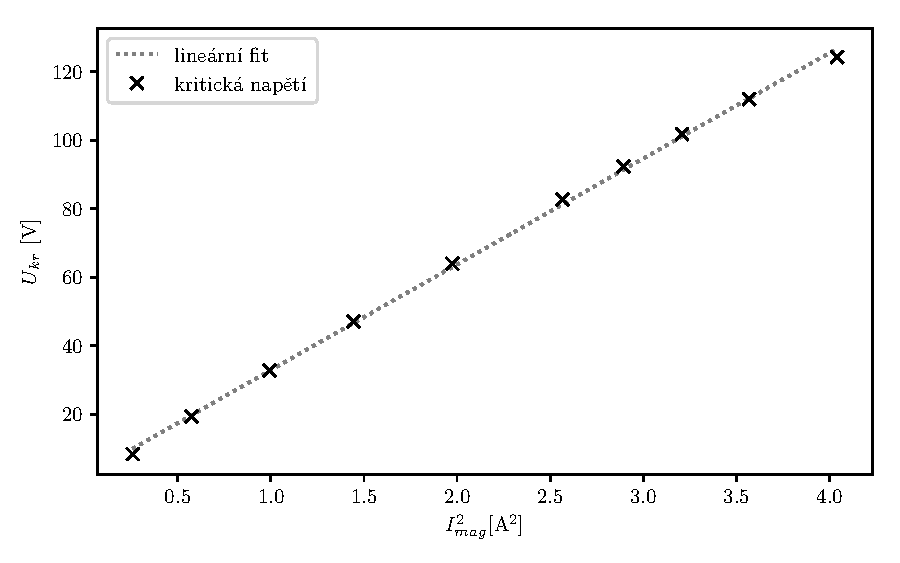
\includegraphics[]{u2}
%            \caption{Graf závislosti ionizačního proudu na přiloženém napětí pro $d = 2$ a $ \SI{6}{cm}$}
%            \label{fig:u2}
%        \end{minipage}
%    \end{figure}

    Je zřejmé, že první část grafu~\ref{fig:u2}, kde proud prudce roste s napětím je oblast Ohmova zákona, druhá část oblast nasyceného proudu. Z teorie vyplývá, že optimální napětí je v oblasti nasyceného proudu, volíme proto $U = \SI{500}{V}$, a že je vhodnější použít větší vzdálenost elektrod, proto volíme $d = \SI{6}{cm}$. Pro srovnání byly proměřeny proudy při optimálním napětí pro všechny možné vzdálenosti elektrod, výsledky jsou uvedeny v tabulce \ref{tab:u3}.

%    \begin{wraptable}[13]{R}{0.25\textwidth}
%        \centering
%        \setlength{\tabcolsep}{10pt}
%        \begin{tabular}[t]{
  S[table-format=1.0]
  S[table-format=2.1]
} \toprule
{$d$}  & {$I$}  \\
{[cm]} & {[nA]} \\ \midrule
     2 & 6.9 \\
     3 & 10.5 \\
     4 & 12.5 \\
     5 & 12.5 \\
     6 & 12.5 \\ \bottomrule
\end{tabular}
%        \caption{Závislost proudu na vzdálenosti elektrod}
%        \label{tab:u3}
%    \end{wraptable}

    Následně byl změřen svodový proud, tj. proud bez přítomnosti zdroje záření, pro $U = \SI{500}{V}$ a optimální vzdálenost elektrod
    \[ I_{svod} = \SI{0.03 \pm 0.05}{pA},\]
    což je hodnota v rámci chyby shodná s nulou. Proto bylo upuštěno od měření celé charakteristiky.


    Pomocí osciloskopu byla změřena závislost amplitudy elektrického impulzu Geiger-Müllerova detektoru na napětí v rozsahu $800-\SI{1500}{V}$. Pro nižší hodnoty napětí nebyla pozorována odezva. Výsledky jsou uvedeny v tabulce  a zobrazeny v grafu . První část grafu je zřejmě oblast nasyceného proudu, následovaná oblastí lavinového zesílení, ve které jsou nosiče náboje urychleny natolik, že sami ionizují. Geiger-Müllerovy oblasti nebylo dosaženo.


    \section*{Diskuse}

    Hodnoty ionizačního proudu poměrně výrazně kmitaly, nebylo proto snadné určit správnou hodnotu a tomu odpovídají chyby hodnot. Hodnoty vzdáleností $d$ byly považovány za přesné.

    Z důvodu malé citlivosti osciloskopu nebylo možné proměřit celou voltampérovou charakteristiku Geiger-Müllerova detektoru, chybí v ní proto úseky Ohmova zákona a nasyceného proudu.

    \section*{Závěr}

    Silnějším zářičem je zářič EA14. Změřené voltampérové charakteristiky odpovídají teoretickým předpovědím a byly náležitě popsány. Byly nalezené optimální podmínky pro měření s ionizační komorou.


    \begin{thebibliography}{}

        \bibitem{pokyny}
        Pokyny k měření ``Studium plynových detektorů'', dostupné z\\ \url{https://physics.mff.cuni.cz/vyuka/zfp/_media/zadani/texty/txt_402.pdf}, 24.\,10.\,2018

    \end{thebibliography}

\end{document}